\documentclass{proseminar}

\begin{document}

\conferenceinfo{Albert-Ludwigs Universit\"at Freiburg\\Technische Fakult\"at, Institut f\"ur Informatik\\Lehrstuhl f\"ur Datenbanken \& Informationssysteme}{}

\title{Trust and Privacy in Social Media \\
\huge Content oriented trust}

\numberofauthors{1} 
\author{
Tim Schmiedl\\
\email{tim.schmiedl@neptun.uni-freiburg.de}
}

\maketitle

\section{Introduction}
* Microblogging is a well-established paradigm for interaction in online social networks. 

* real-time fashion 

* mobile internet devices 

* propagating news and information about developing events 





\subsection*{Current Situation \& Potential}
+ new ranking strategy that considers popularity of tweets

* Besides helping to communicate relevant events on a day-to-day basis, microblogging can be particularly helpful during emergency and/or crisis
situations 

* provide real-time information from the actual location where the crisis is unfolding. This
information often spreads faster and to a wider audience than what traditional news
media sources can achieve.




\subsection*{Problems}
+ This ranking method, however, has not taken into account content relevance or the twitter account.

+ a large amount of pointless tweets may flood the relevant tweets

+ spam is not avoided in rankin method

* variety of content; NEWS / Chat

* valuable to the user and its immediate circle offriends VS  valuable to a broader community

* NO DISTINCTION between news / chat




\subsection*{Goals of the Papers}
+ In this paper,  a method to rank the tweets  based on their content relevance to the query

+  learning to rank approach

+  best set of features

* In this work we focus mostly on the credibility of newsworthy information is a correlation between how information propagates and the credibility 

* aid them in the process of discovering reliable information.  achieved in an automatic way using features extracted from information cascades





\section{Twitter Case Study}
* from P1: Predicting information credibility in time-sensitive social media

* earthquake that hit Chile on February 2010

*  Event characterization

*  Twitter reaction: Information propagation behavior \& False rumor propagation

\section{Retrieving and Labeling of Data}



\section{Ranking of Tweets}
+ method of P2: An Empirical Study on Learning to Rank of Tweets

+ Learning to Rank: data-driven approach

+ RankSVM for training the ranking model

\begin{figure}[h]
\centering
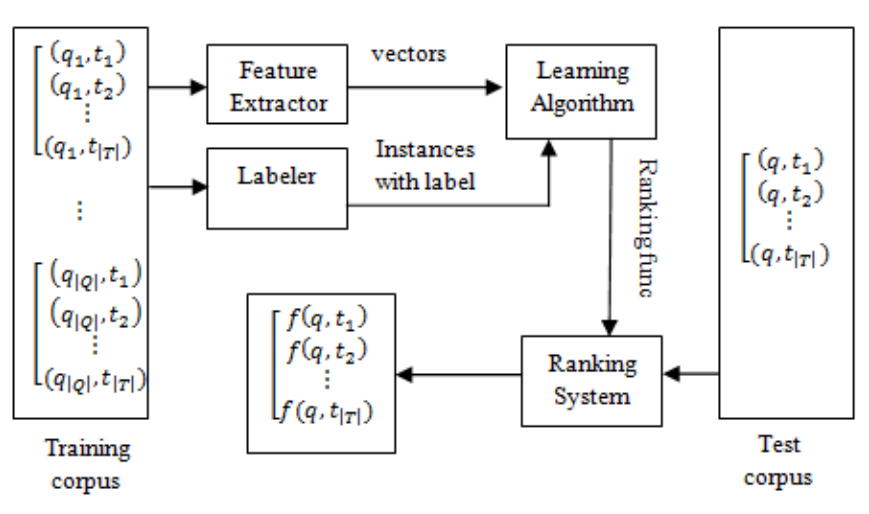
\epsfig{file=img/p2_overview.png, width=0.45\textwidth}
\caption{General Paradigm of Learning for Tweets Ranking}
\end{figure}

+ Features for Ranking: Content relevance features, Twitter specific features, Account authority features

\paragraph{Content relevance features}

+ three differen content relevance features

+ Okapi BM25: content relevance between query and tweet

+ Similarity  of  contents: cosine sim for pair of tweets

+ Length: number of words

\paragraph{Content relevance features}


\section{Prediction Model for Tweets}



\section{Evaluation}



\section{Related Work}



\section{Conclusion}



\bibliographystyle{abbrv}
\bibliography{bibliography}  

\balancecolumns

\end{document}
